% Importamos el preámbulo con la configuración del documento
% Definición de la clase del documento
\documentclass[a4paper, 11pt]{book} % A4 paper and 11pt font size

% Entrada y salida de texto
\usepackage[T1]{fontenc}
\usepackage[utf8]{inputenc}
\usepackage[sfdefault]{roboto} % Option 'sfdefault' only if the base font of the document is to be sans serif

% Idioma
\usepackage[spanish, es-tabla]{babel} % Selecciona el español y el uso de la palabra "tabla" en lugar de "cuadro"

% Información reutilizable
\newcommand{\asunto}{Trabajo de Fin de Grado}
\newcommand{\titulo}{Juego de tablero aumentado utilizando ARCore}
\newcommand{\tituloEng}{Augmented board game using ARCore}
\newcommand{\subtitulo}{Desarrollo de un juego de mesa aumentado mediante uso de tecnologías de realidad aumentada}
\newcommand{\subtituloEng}{Development of augmented board game using augmented reality technologies}
\newcommand{\grado}{Grado en Ingeniería Informática}
\newcommand{\autor}{Miguel Ángel Torres López}
\newcommand{\email}{matl1995@correo.ugr.es}
\newcommand{\tutor}{Francisco Luis Gutiérrez Vela}
\newcommand{\escuela}{Escuela Técnica Superior de Ingenierías Informática y de Telecomunicación}
\newcommand{\departamento}{Departamento de Lenguajes y Sistemas Informáticos}
\newcommand{\universidad}{Universidad de Granada}
\newcommand{\ciudad}{Granada}
\providecommand{\keywords}{ARCore, Unity, Android, juegos de mesa}
\providecommand{\keywordsEng}{ARCore, Unity, Android, board games}

% Otros paquetes importantes para el proyecto
\usepackage[hyphens]{url}
\usepackage{eurosym}
\usepackage{graphicx}
\usepackage{colortbl}
\usepackage{fancyhdr}
\usepackage{pdfpages}
\usepackage{longtable}
\usepackage[hidelinks]{hyperref}
\usepackage{placeins}
\usepackage{verbatim}

\setcounter{tocdepth}{4}
\setcounter{secnumdepth}{4}

% Añade aquí las carpetas de imágenes para que el compilador las pueda analizar
\graphicspath{{../images/}{../screenshots/}{../images/applications/}{../images/integration/}{../images/techniques/}{../images/mockups/}{../images/headmounted/}{../images/tangibleinterfaces/}{../images/estudiomercado1/}{../images/estudiomercado2/}{../images/metodologias/}{../images/desarrollo/}{../images/entrega2/}}

% Información del archivo
\hypersetup{
  pdfauthor = {\autor\ (\email)},
  pdftitle = {\titulo: \subtitulo},
  pdfsubject = {\asunto},
  pdfkeywords = {\keywords},
  pdfcreator = {LaTeX, con la distribución TeX Live},
  pdfproducer = {pdflatex}
}

% Modificación para que las páginas en blanco no tengan cabecera
\makeatletter
\def\clearpage{
  \ifvmode
    \ifnum \@dbltopnum = \m@ne
      \ifdim \pagetotal < \topskip
        \hbox{}
      \fi
    \fi
  \fi
  \newpage
  \thispagestyle{empty}
  \write\m@ne{}
  \vbox{}
  \penalty -\@Mi
}
\makeatother

% Definición del estilo de las cabeceras
\pagestyle{fancy}
\fancyhf{}
\fancyhead[LO]{\leftmark}
\fancyhead[RE]{\rightmark}
\fancyhead[RO,LE]{\textbf{\thepage}}
\setlength{\headheight}{1.5\headheight}

% Definición de colores
\definecolor{Gray}{gray}{0.9}

% Redefinición de comandos
\renewcommand{\chaptermark}[1]{\markboth{\textbf{#1}}{}}
\renewcommand{\sectionmark}[1]{\markright{\textbf{\thesection. #1}}{}}
% \renewcommand{\lstlistingname}{Fragmento de código}
% \renewcommand{\lstlistlistingname}{Índice de fragmentos de código}

% Creación de comandos
% \newcommand{\HRule}{\rule{\linewidth}{0.5mm}}
% \newcommand{\bigrule}{\titlerule[0.5mm]}

% Ajuste para minimizar el fragmentado de listados
% \lstnewenvironment{listing}[1][]
%   {\lstset{#1}\pagebreak[0]}{\pagebreak[0]}


\begin{document}

% Portada del documento
\begin{titlepage}

\newlength{\centeroffset}
\setlength{\centeroffset}{-0.5\oddsidemargin}
\addtolength{\centeroffset}{0.5\evensidemargin}

\noindent\hspace*{\centeroffset}

\begin{minipage}{\textwidth}

\centering


\includegraphics[width=0.9\textwidth]{logo_ugr}\\[1.4cm]

\textsc{\Large\asunto\\[0.2cm]}
\textsc{\grado}\\[1cm]

{\Huge\bfseries\titulo\\}
\noindent\rule[-1ex]{\textwidth}{3pt}\\[3.5ex]
{\large\bfseries\subtitulo}

\end{minipage}

\vspace{1.5cm}
\noindent\hspace*{\centeroffset}

\begin{minipage}{\textwidth}

\centering

\textbf{Autor}\\{\autor}\\[2.5ex]
\textbf{Tutor}\\{\tutor}\\[1.5cm]


\includegraphics[width=0.3\textwidth]{logo_etsiit}\\[0.1cm]

\textsc{\escuela}\\
\textsc{---}\\
\ciudad, \today\\

\end{minipage}

\end{titlepage}


% Prefacio del documento
\cleardoublepage
\thispagestyle{empty}

\begin{center}
{\LARGE\bfseries\titulo: \subtitulo}\\
\end{center}
\begin{center}
\autor
\end{center}

\bigskip
\noindent{\textbf{Palabras clave}: \textit{\keywords}\\

\section*{Resumen}
Este documento expone mi trabajo de fin de grado, y los contenidos asociados al mismo.\\

Este proyecto se va a centrar en la planificación y desarrollo de un juego de mesa, que mediante las tecnologías de realidad aumentada, mas concretamente ARCore, aportará un nuevo enfoque sobre los juegos de esta temática, aprovechando las singulares características que la realidad aumentada ofrece.\\

El objetivo principal del juego es explorar que ventajas puede aportar la realidad aumentada a los juegos en dispositivos móviles, y mas específicamente a los juegos de mesa en dispositivos móviles.\\

El proyecto explorará también la integración de diferentes formas de interacción en juegos, permitiendo funcionalidades que se tendrán que llevar a cabo mediante interacción con elementos físicos, y otras funcionalidades que se desarrollarán con interacción únicamente con el dispositivo móvil.\\

\cleardoublepage
\thispagestyle{empty}

\begin{center}
{\LARGE\bfseries\tituloEng: \subtituloEng}\\
\end{center}
\begin{center}
\autor
\end{center}

\bigskip
\noindent{\textbf{Keywords}: \textit{\keywordsEng}\\

\section*{Abstract}
This document shows my end-of-degree project and the contents associated with it.\\

This project will focus on the planning and development of a board game, that using the augmented reality technologies available, specifically using ARCore, will bring a new approach to the games of this theme, taking advantage of the singular characteristics that augmented reality offers.\\

The main objective of the game is to explore the advantages that augmented reality can bring to mobile devices games, and more specifically to board games in mobile devices.\\

The project will also explore the integration of different ways of interaction in games, allowing functionalities that will have to be done by interacting with physical elements, and other functionalities that will have to be done interacting only with the mobile device.\\

\chapter*{}
\thispagestyle{empty}

\noindent\rule[-1ex]{\textwidth}{2pt}\\[4.5ex]

Yo, \textbf{\autor}, alumno de la titulación \textbf{\grado} de la \textbf{\escuela} de la \textbf{\universidad}, con DNI 71358141C, autorizo la ubicación de la siguiente copia de mi Trabajo de Fin de Grado en la biblioteca del centro para que pueda ser consultada por las personas que lo deseen.\\

Así mismo, el código fuente del proyecto y esta documentación pueden consultarse en la dirección \url{https://github.com/matl1995/TFG} para que aquellos que lo deseen puedan probar el proyecto.

\vspace{5cm}

\noindent \textbf{Fdo: \autor}

\vspace{2cm}

\begin{flushright}
\ciudad, a \today
\end{flushright}

\chapter*{}
\thispagestyle{empty}

\noindent\rule[-1ex]{\textwidth}{2pt}\\[4.5ex]

D. \textbf{\tutor}, profesor del \textbf{\departamento} de la \textbf{\universidad}.

\vspace{0.5cm}

\textbf{Informa:}

\vspace{0.5cm}

Que el presente trabajo, titulado \textit{\textbf{\titulo: \subtitulo}}, ha sido realizado bajo su supervisión por \textbf{\autor}, y autoriza la defensa de dicho trabajo ante el tribunal que corresponda.

\vspace{0.5cm}

Y para que conste, expide y firma el presente informe en \ciudad, a \today.

\vspace{1cm}

\textbf{El tutor:}

\vspace{5cm}

% \begin{figure}[H]
% \includegraphics[width=0.3\textwidth]{firma_tutor}
% \end{figure}

\noindent\textbf{\tutor}

\chapter*{Agradecimientos}
\thispagestyle{empty}

\vspace{1cm}

A mi tutor del TFG por toda la ayuda y apoyo durante el proyecto.\\

A mi familia por estar ahi siempre que lo he necesitado.\\

A mis amigos y amigas por todas las veces que me han ayudado y apoyado durante todas las etapas de mi vida.\\

A mis profesores por su incansable esfuerzo durante estos años de carrera para que aprendamos lo máximo posible y de la mejor manera.\\


\frontmatter
\begingroup
\let\cleardoublepage\clearpage
  \tableofcontents
  % \listoffigures
  % \listoftables
  % \lstlistoflistings
\endgroup

\newpage
\thispagestyle{empty}

% Capítulos del documento
\mainmatter
\chapter{Introducción y objetivo}
\label{ch:introduccion}

\section{Introducción}
La realidad aumentada es una tecnología que está en pleno auge, no paramos de ver noticias que nos muestran todo lo que esta permite, las diferentes utilizades que tiene y como va a mejorarnos la vida. No obstante esto no era así hace un año, como se puede observar en el grafico del "Hype Cycle" de Gartner sobre tecnologías emergentes en 2017, Figura \ref{figura-gartner}, la realidad aumentada se situaba en el tramo de desilusión, lo que significa que despues de estar en lo alto de la gráfica años anteriores, cuando se hablaba mucho de la tecnología y todo lo que ofrecía, en julio de 2017 se encontraba en lo mas bajo, apenas se hablaba de dicha tecnología, lo que significa que aun hay mucho por hacer, y queda mucho por trabajar sobre esta tecnología.\\

\begin{figure}[h]
  \centering
  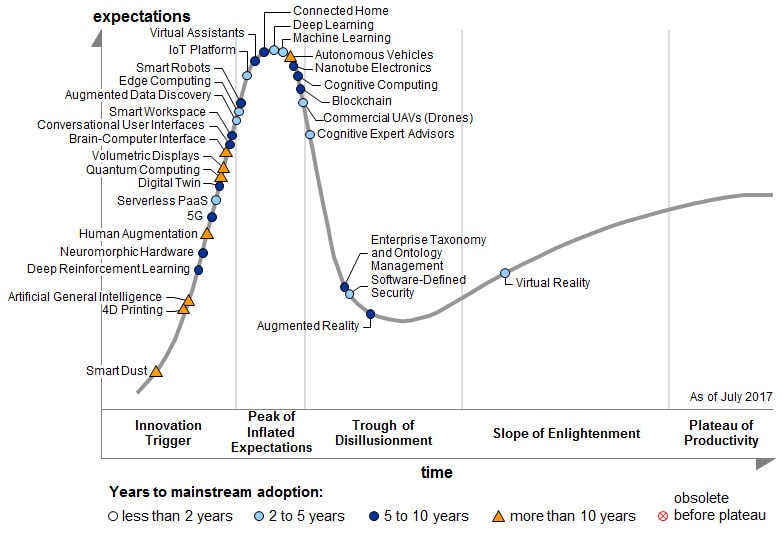
\includegraphics[scale=0.5]{gartner-hype-cycle}
  \caption{Imagen que muestra el "Hype cycle" de Gartner para tecnologías emergentes en 2017.\protect\footnotemark}
  \label{figura-gartner}
\end{figure}

\footnotetext{ \url{https://www.gartner.com/newsroom/id/3784363}, Gartner (July 2017)}

Sin embargo, desde que Apple y Google lanzaran sus respectivas librerías hace apenas un año, la realidad aumentada ha mejorado su situación notablemente, distanciándose de la realidad aumentada vista hasta el momento, estas nuevas librerias permiten, con los componentes de un dispositivo móvil de masas sea posible reconocer y entender el mundo que le rodea, así como su posición en el mundo. Esto supone una diferenciación en las tecnologías hasta entonces presentes, que o bien necesitaban de mucho hardware para ser capaces de conseguir esto, o en dispositivos móviles de masas, tenían capacidades reducidas.\\

Actualmente la realidad aumentada abre un mundo de grandes posibilidades que pueden revolucionar muchos ámbitos, entre ellos el de los juegos, un juego ya no tiene que quedarse dentro de una pantalla o un mundo virtual, ahora puede dar el salto el mundo real, esto aporta un grado de realismo y espectacularidad que puede suponer una reinvención de los juegos como ahora los conocemos.\\

Por otro lado, la mayoría de la población dispone de un dispositivo móvil, como podemos ver en la Figura \ref{figura-ine}, en el año 2017, un 97.4\% de los hogares españoles contaba con al menos un dispositivo móvil \cite{ine}, esto implica que casi la totalidad de los españoles tiene acceso a dispositivos móviles, y por tanto, a las aplicaciones que utilizan realidad aumentada.

\begin{figure}[h]
  \centering
  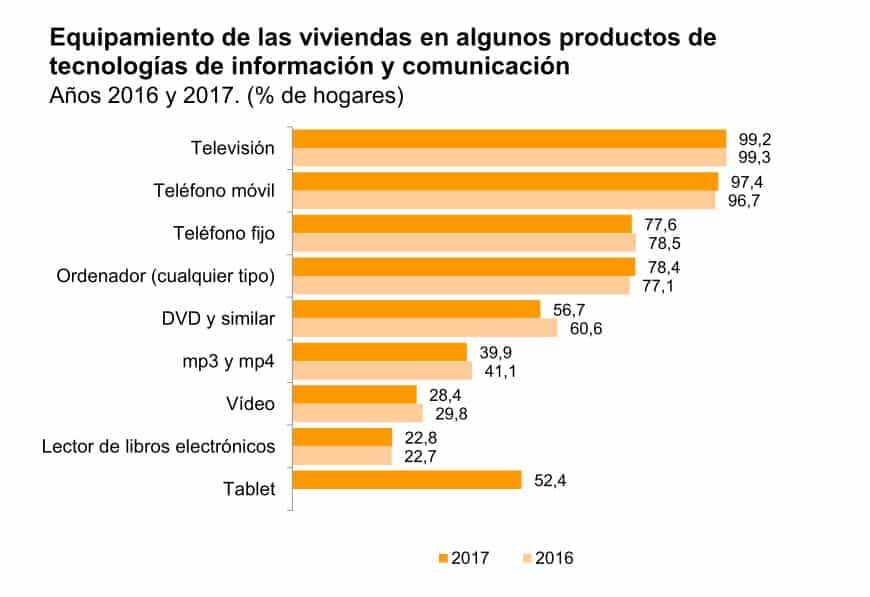
\includegraphics[scale=0.4]{ine2017}
  \caption{Imagen que muestra los porcentajes de hogares que cuentan con cada dispositivo tecnológico.\protect\footnotemark}
  \label{figura-ine}
\end{figure}

\footnotetext{{\em Encuesta sobre Equipamiento y Uso de Tecnologías de la Información y Comunicación en los Hogares.} INE, B. (2017).}

\newpage

\section{Motivación}
Personalmente el estar una gran parte del tiempo de cada dia utilizando mi teléfono móvil y jugando con el me despertó la curiosidad acerca de como se desarrollan los videojuegos, y que es lo que hay detras del producto que al final el usuario descarga de una tienda de aplicaciones.\\

Por otro lado, mi interés por el desarrollo del software me lleva a querer conocer y explorar este mundo, la experiencia de planificar y desarrollar un proyecto software al completo por mi mismo.\\

Las nuevas tecnologías siempre me han llamado la atención y me gusta estar informado sobre ellas, y viendo la revolución de la realidad aumentada me pareció un mundo apasionante por las capacidades ofrece, el poder fusionar el mundo virtual y real, y llevar a cabo aplicaciones y juegos con ella, me pareció algo fascinante y que sin duda me gustaría explorar.\\

La amplia disponibilidad de dispositivos móviles entre la población, y el alto nivel de uso diario que hacen los usuarios de estos, hace del desarrollo para estos dispositivos algo atractivo, ya que es probablemente la mayor plataforma para desarrolladores de software actualmente.\\

Esto en conjunto con el crecimiento de la realidad aumentada, hace que un juego para dispositivos móviles que hace uso de esta tecnología, sea una opción muy interesante para un proyecto, que permite adquirir conocimientos en el desarrollo de videojuegos, en el desarrollo de aplicaciones móviles, y exploarar la realidad aumentada y lo que puede aportar a las aplicaciones de dispositivos móviles actuales.

\section{Estructura del documento}
Este documento se divide en 4 capítulos, a continuación se detalla el contenido de cada uno de los capítulos del documento:
\begin{itemize}
  \item \textbf{Capítulo 1, Introducción y objetivo:} En este capítulo se hace una pequeña introducción al proyecto, explicando la motivación por la que surgió el proyecto, la estructura del documento, y también se exponen los objetivos que han sido establecidos para este proyecto.
  \item \textbf{Capítulo 2, Estado del arte:} En este capítulo se hará una exposición de cual es el estado actual de la realidad aumentada, diferencias con tecnologías similares, que aplicaciones tiene, etc.
  \item \textbf{Capítulo 3, Análisis inicial del problema:} En este capítulo se llevará acabo un analisis de cual es el problema y como este puede ser resuelto.
  \item \textbf{Capítulo 4, Metodologías a usar en el proyecto:} En este capítulo se recogen las diferentes metodologías utilizadas para el desarrollo del proyecto, y se explica como serán utilizadas en el proyecto.
  \item \textbf{Capítulo 5, Plan de entregas:} En este capítulo se detalla el plan de entregas llevado a cabo, y las historias de usuario realizadas para definir los requisitos que tendrá el sistema.
  \item \textbf{Capítulo 6, Desarrollo. Entregas e iteraciones:} En esta capitulo se recogerá el trabajo realizado durante las diferentes iteraciones, así como el resultado de las distintas entregas.
  \item \textbf{Capítulo 7, Conclusiones y Trabajos Futuros:} En este capítulo se recoge el resultado del proyecto, las conclusiones obtenidas del desarrollo de éste y los trabajos futuros a realizar en el proyecto.
\end{itemize}

\section{Objetivo}
El objetivo principal de este proyecto es explorar que ventajas puede aportar la realidad aumentada, mas concretamente el SDK ARCore, a los juegos en dispositivos móviles, y mas específicamente a los juegos de mesa en dispositivos móviles. Por tanto, mediante este proyecto se adquirirá experiencia en el desarrollo con tecnologías de realidad aumentada.\\

Objetivos secundarios:
\begin{itemize}
  \item Investigar una implementación para juegos de mesa virtuales que aporte un enfoque diferente al habitual.
  \item Adquirir conocimientos sobre la planificación y desarrollo de proyectos de software, mas concretamente de videojuegos.
  \item Adquirir conocimientos sobre la realidad aumentada, como ésta funciona y cuales son las mejores SDK para desarrollar utilizando dicha tecnología.
\end{itemize}

\chapter{Objetivos}
\label{ch:objetivos}

\chapter{Estado del arte}
\label{ch:estado}

\section{Realidad aumentada}
Una de las primeras definiciones de realidad aumentada fue dada por Ronald Azuma en 1997 \cite{azuma}, y dice que la Realidad Aumentada es cualquier sistema que combine elementos reales y virtuales, que sea interactivo en tiempo real y que sea registrado en tres dimensiones. Por tanto, la realidad aumentada es una tecnología que permite añadir información virtual al mundo real a través de un dispositivo, es decir, permite mostrar el mundo real con objetos virtuales en éste, por lo que no pretende crear un mundo virtual, sino complementar al mundo real con más información.

\section{Diferencias entre realidad aumentada, realidad virtual y realidad mixta}
\textbf{Realidad virtual}: Es una tecnología completamente inmersiva que consiste en convencer a tus sentidos de que estas en otro mundo que no es el real, es un mundo virtual. Usando un dispositivo que se coloca en la cabeza, la realidad virtual permite disfrutar de un mundo de imágenes y sonidos generado por ordenador en el que se puede manipular objetos, y moverse por dicho mundo usando controladores hápticos conectados a un ordenador o a una consola. \cite{intel}

\textbf{Realidad aumentad}a: Es una tecnología que superpone información digital sobre elementos del mundo real. El elemento central es el mundo real, pero lo mejora con otros detalles digitales, complementando así la realidad. \cite{intel}

\textbf{Realidad mixta}: Es una tecnología que hace converger el mundo real y elementos digitales. En esta puedes interactuar y manipular tanto elementos físicos como virtuales. La realidad mixta te permite sumergirte en el mundo que te rodea incluso cuando tú interactúas con el entorno virtual usando tus propias manos. Esta tecnología te permite tener un pie en el mundo real y el otro en un lugar imaginario. \cite{intel}

\section{Aplicaciones de la realidad aumentada}
\begin{itemize}
  \item \textbf{Medicina}: La realidad aumentada puede aportar grandes avances a la medicina, ya que permite la visualización en 3D de objetos que bien pueden ser órganos o partes del cuerpo en el mundo real, por lo que puede facilitar a los doctores muchas tareas que requieran el estudio de modelos 3D. Por ejemplo, los doctores pueden utilizar la realidad aumentada con el objetivo de prepararse para una operación como se puede observar en la Figura \ref{figura-medicina}, o simplemente para tareas de visualización médica, de igual manera que actualmente se utilizan los TAC o las resonancias magnéticas, pero los datos obtenidos con dichos escáneres se convertirían en modelos 3D que son mucho más sencillos de explorar que un conjunto de imágenes 2D. También se podría utilizar la realidad aumentada con el objetivo de entrenamiento para cirujanos que se están formando, mostrándoles instrucciones sobre un modelo 3D de cómo se debería realizar una determinada operación, ayudando así a que no necesiten consultar un manual y quitar la vista del “paciente” si no que todo sería sobre dicho “paciente” que realmente es un modelo 3D. \cite{azuma}

  \begin{figure}[h]
    \centering
    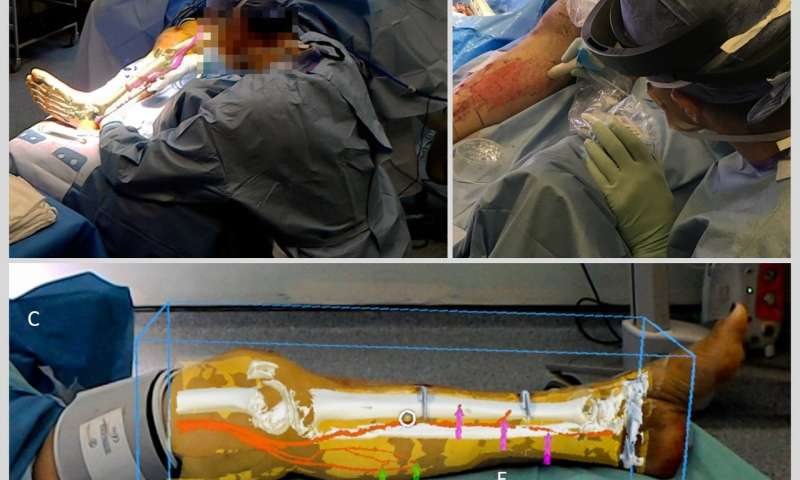
\includegraphics[scale=0.5]{medicine}
    \caption{Profesionales médicos utilziando realidad aumentada como ayuda para una operación.\protect\footnotemark}
    \label{figura-medicina}
  \end{figure}

  \footnotetext{ Philip Pratt, et al. Eur Radiol Exp, 2018}

  \newpage

  \item \textbf{Educación}: La realidad aumentada tiene mucho que aportar a la educación, ya que permite una forma interactiva de aprender que los libros no permiten. Por ejemplo, que mejor manera de aprender el sistema respiratorio que con uno a tamaño real en 3D que tu puedes explorar. Y la realidad aumentada no implica que los libros no sirvan y vayan a desaparecer, si no que puede suponer un complemento para dichos libros como se puede observar en la Figura \ref{figura-educacion}, cambiando la forma en la que nos relacionamos con ellos, por ejemplo, con imágenes en los libros que al escanearlas muestren elementos 3D que nos permitan comprender mejor el contenido que se está exponiendo en dicho libro. \cite{reinoso}

  \begin{figure}[h]
    \centering
    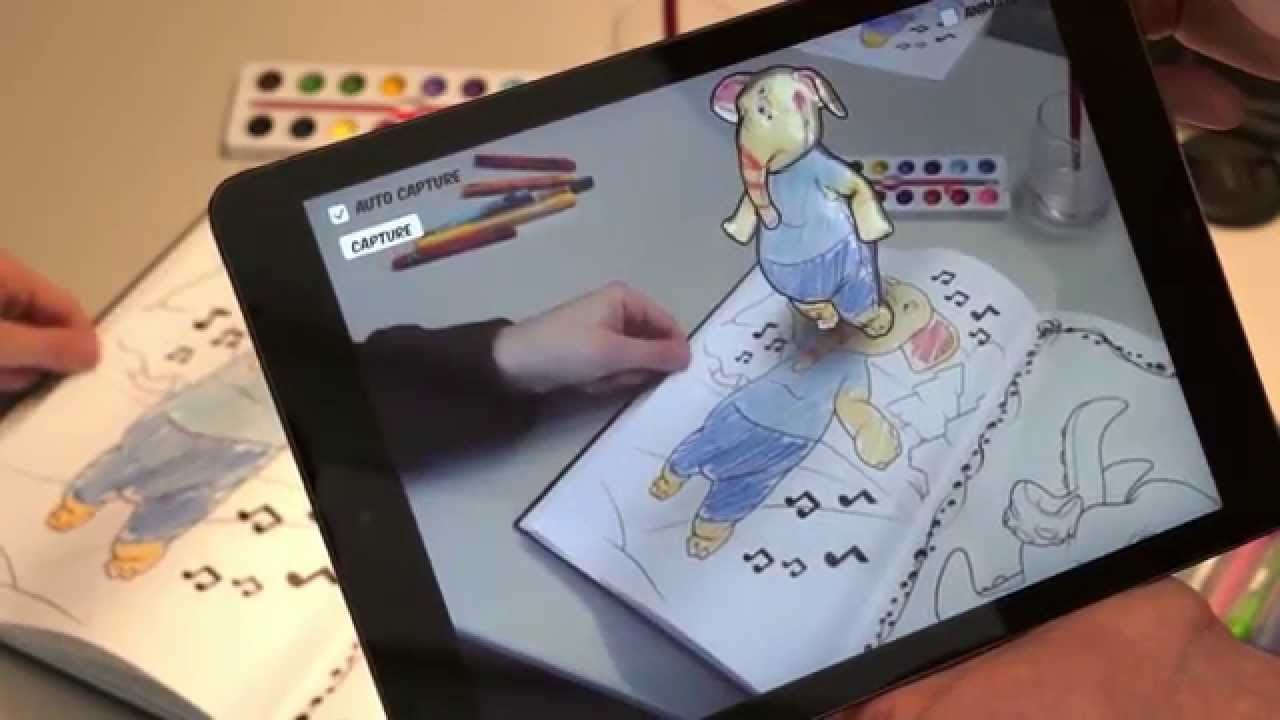
\includegraphics[scale=0.2]{education}
    \caption{Libro que utiliza la realidad aumentada para mostrar el dibujo en 3D.\protect\footnotemark}
    \label{figura-educacion}
  \end{figure}

  \footnotetext{ \url{https://www.youtube.com/watch?v=IeHKVC0XLe4}, Alibabach}

  \begin{figure}[h]
    \centering
    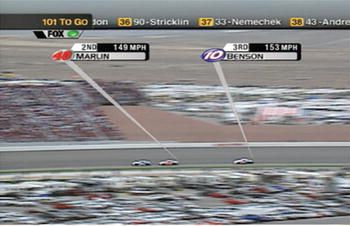
\includegraphics[scale=0.7]{entertainment1}
    \caption{Imagen que muestra la utilización de realidad aumentada en la retransmisión de deportes. \cite{van-krevelen}}
    \label{figura-entretenimiento1}
  \end{figure}

  \item \textbf{Entretenimiento}: La realidad aumentada se puede aplicar en el entretenimiento relacionada a juegos, por ejemplo, mostrando los tableros de juego en una superficie plana en lugar de en la pantalla en 2D, como se puede ver en la Figura \ref{figura-entretenimiento}, pero también se puede aplicar la realidad aumentada en otras formas de entretenimiento diferentes, por ejemplo, en los deportes que se retransmiten, mostrando información relevante para los usuarios sobre dicho deporte, por ejemplo, en las carreras de coches, ya que puede estar grabado desde cierta distancia mostrar sobre cada coche información de quien es, su puesto y la velocidad que lleva como se puede ver en la Figura \ref{figura-entretenimiento1}. \cite{van-krevelen}

  \begin{figure}[h]
    \centering
    
\includegraphics[scale=0.1]{entertainment}
    \caption{Imagen que muestra la utilización de realidad aumentada en un juego.\protect\footnotemark}
    \label{figura-entretenimiento}
  \end{figure}

  \footnotetext{ \url{https://itunes.apple.com/us/app/stack-ar/id1269638287?mt=8}, Ketchapp}

  \item \textbf{Turismo}: La realidad aumentada puede dar una vuelta al turismo, teniendo un guia turistico en tu propio dispositivo móvil, por ejemplo, mediante el uso de realidad aumentada que utiliza la geolocalización, puede indicar los monumentos relevantes de la ciudad, la distancia a ellos y donde están a través de la cámara de un dispositivo móvil. También puede mejorar las experiencias turísticas actuales de una forma mucho más visual, cuando se esté en un sitio histórico te puede contar la historia de una forma más entretenida y visual, mostrando elementos 3D en el lugar, recreando lo que sucedió, como se puede observar en la Figura \ref{figura-turismo}. \cite{reinoso}

  \begin{figure}[h]
    \centering
    
\includegraphics[scale=0.15]{turism}
    \caption{Imagen que muestra un hecho historico visualizandose con realidad aumentada. \cite{layar}}
    \label{figura-turismo}
  \end{figure}

  \newpage

  \item \textbf{Comercio}: La realidad aumentada puede revolucionar el sector de las ventas por internet, la mayor desventaja actual que tiene comprar por internet es que el usuario se tiene que conformar con imágenes 2D del producto, la realidad aumentada permite romper esa barrera, y mostrar al usuario el producto en 3D, en tamaño real en su propia casa, por ejemplo, esto es muy útil con muebles ya que necesitas las medidas del hueco que tienes y del mueble para saber si encajará en el hueco o simplemente si queda bonito en la habitación, con la realidad aumentada ambos problemas están solucionados, puedes ver el mueble en el hueco que quieres en tamaño real, lo que te permite saber si cabe y si queda bien. Un ejemplo de este tipo de aplicación se puede observar en la Figura \ref{figura-comercio}.

  \begin{figure}
    \centering
    
\includegraphics[scale=0.3]{commerce}
    \caption{Imagen que muestra la utilización de realidad aumentada en un juego.\protect\footnotemark}
    \label{figura-comercio}
  \end{figure}

  \footnotetext{ \url{https://itunes.apple.com/es/app/ikea-place/id1279244498?mt=8}, Ikea}

\end{itemize}

\newpage

\section{Formas de integrar la información digital con el mundo real \cite{prendes-espinosa}}

\begin{itemize}
  \item \textbf{Vincular la información a un marcador}: Un marcador es una imagen en blanco y negro que contiene un patrón, como puede ser un código QR, un ejemplo de marcador se puede ver en la Figura \ref{figura-marcador}. Este tipo de tecnologóia almacena en memoria marcadores, y cuando se escanea dicho marcador se puede mostrar una información asociada a este con respecto a la posición de dicho marcador, como se puede ver en la Figura \ref{figura-marcador-aumentado}.

  \begin{figure}
    \centering
    
\includegraphics[scale=0.3]{marker}
    \caption{Imagen que muestra un ejemplo de marcador.}
    \label{figura-marcador}
  \end{figure}

  \begin{figure}[h]
    \centering
    
\includegraphics[scale=0.5]{marker-augmented}
    \caption{Imagen que muestra un marcador con un modelo 3D asociado a este.}
    \label{figura-marcador-aumentado}
  \end{figure}

  \newpage

  \item \textbf{Vincular la información a una imagen fija o móvil}: Lo que hace es almacenar en memoria imágenes, y cuando dichas imágenes se escanean se puede mostrar una información asociada a dicha imagen con respecto a la posición de la imagen, cabe la posibilidad de que cuando dicha imagen esté en movimiento se pierda la información asociada a esta y se muestre cuando vuelva a estar fija, o por el contrario que dicha información asociada se desplace junto con la imagen. Podemos observar un ejemplo en la Figura \ref{figura-image}.

  \begin{figure}[h]
    \centering
    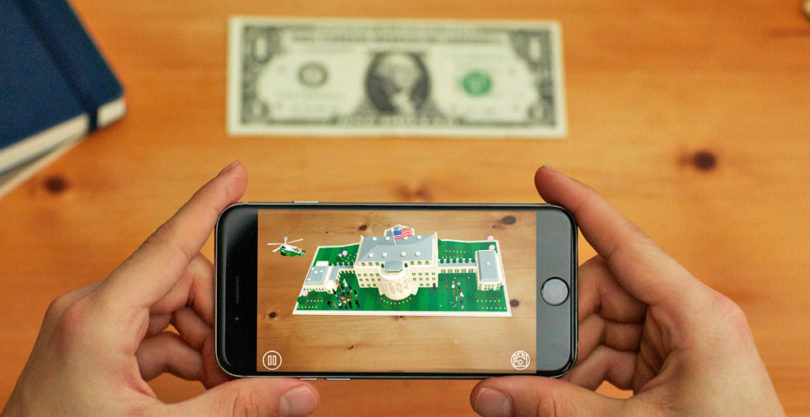
\includegraphics[scale=0.3]{image}
    \caption{Imagen que muestra una imagen con un modelo 3D asociado a esta.\protect\footnotemark}
    \label{figura-image}
  \end{figure}

  \footnotetext{ \url{https://vrscout.com/news/augmented-reality-app-1-dollar-bill-tour-white-house/}, Kyle Melnick}

  \newpage

  \item \textbf{Vincular la información a un objeto 3D}: Lo que ocurre es que se tendrá almacenado en memoria un modelo del objeto, y con dispositivos como Kinect (mostrado en la Figura \ref{figura-kinect}) se puede reconocer dicho objeto y asociar una información a este.

  \begin{figure}[h]
    \centering
    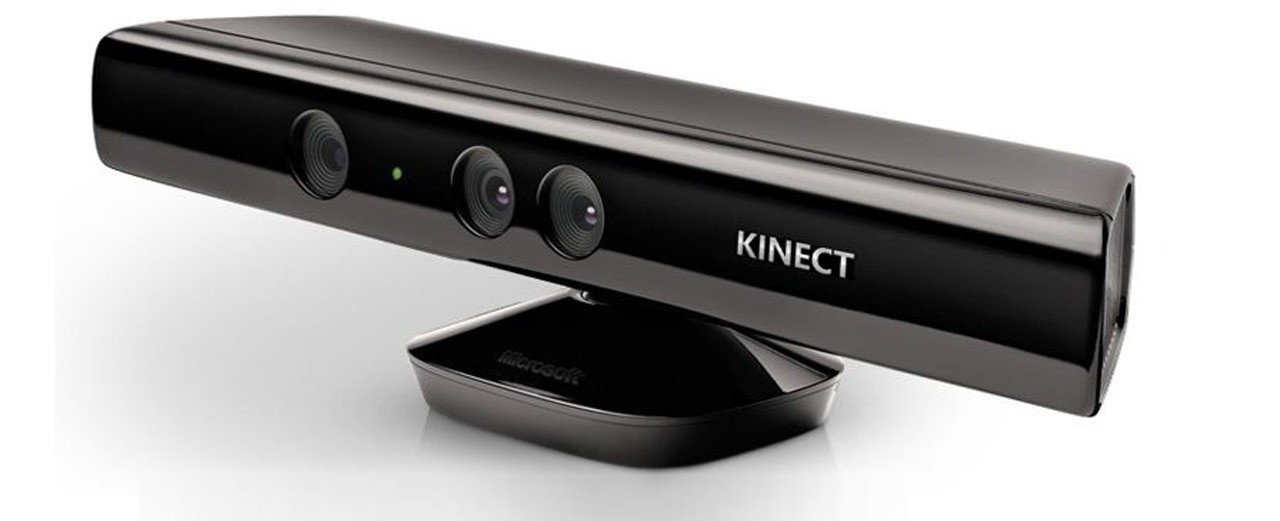
\includegraphics[scale=0.2]{kinect}
    \caption{Imagen que muestra la herramienta kinect.}
    \label{figura-kinect}
  \end{figure}

  \item \textbf{Vincular la información a una escena}:  Lo que hace esta técnica es escanear el mundo real y asignar coordenadas, escaneará las superficies planas horizontales y verticales, y establecerá un modelo 3D de estas, en el que establece coordenadas, y a cada una de estas coordenadas se puede asociar información con respecto a la posición de esta, como se puede ver en la Figura \ref{figura-scene}, lo que nos permitirá gracias a que se escanea el mundo en 3D que al movernos alrededor, incluso si dejamos de tener la coordenada dentro de la visión de la cámara, que al volver a mirar al punto de la coordenada la información asociada siga ahí.

  \begin{figure}[h]
    \centering
    
\includegraphics[scale=0.3]{scene}
    \caption{Imagen que muestra el reconocimiento de superficies de una escena y la asociación de información a una coordenada de esta escena.}
    \label{figura-scene}
  \end{figure}

  \item \textbf{Vincular la información a una coordenada del mundo real}: Se tendrá la información asignada a dicha coordenada del mundo, y gracias al sistema gps del dispositivo y otros sensores, permite que cuando dicha coordenada entre en el rango de visión del dispositivo, muestre la información asociada a esta, como se puede observar en la Figura \ref{figura-location}.

  \begin{figure}[h]
    \centering
    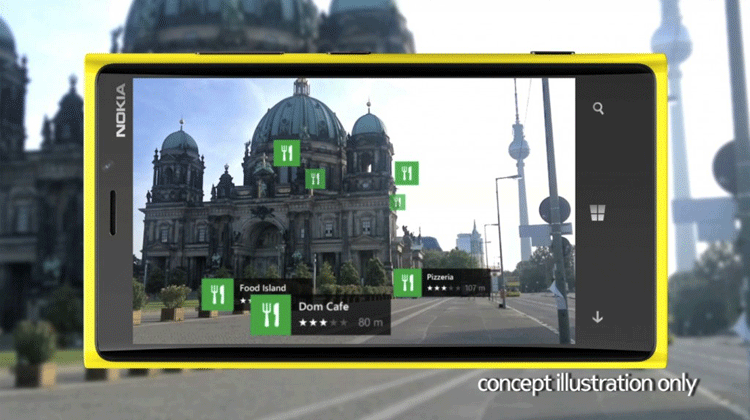
\includegraphics[scale=0.3]{location}
    \caption{Imagen que muestra la visualización de información asociada a coordenadas del mundo real.\protect\footnotemark}
    \label{figura-location}
  \end{figure}

  \footnotetext{ \url{https://www.gislounge.com/augmented-reality-digital-map-revolution/}, Nokia}

\end{itemize}

\section{Dispositivos y técnicas de visualización \cite{billinghurst}}
Existen diferentes tipos de pantallas para la visualización de realidad aumentada:
\begin{itemize}
  \item \textbf{Pantallas basadas en video}: Estas pantallas mediante procesos digitales combinan imágenes virtuales con video del mundo real. Estas pantallas son las más populares al estar en los dispositivos que usamos en el dia a dia como smartphones y tablets, como se puede ver en la Figura \ref{figura-pantalla-video}.

  \begin{figure}[h]
    \centering
    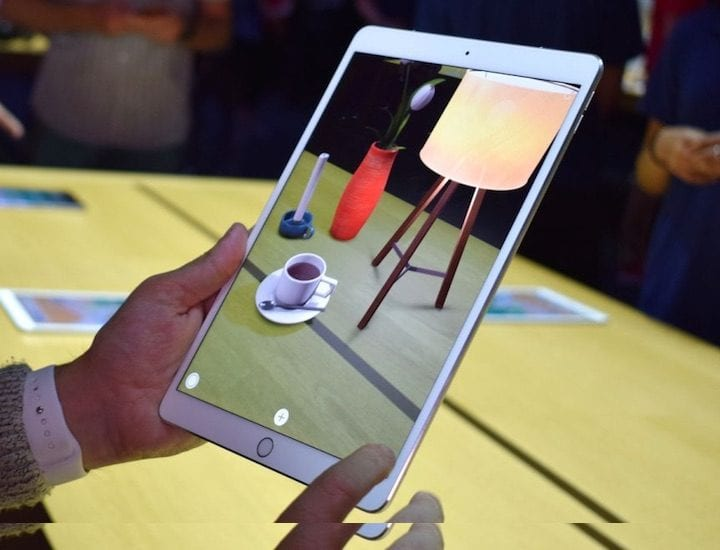
\includegraphics[scale=0.35]{video-screen}
    \caption{Imagen que muestra una tablet usando una aplicación de realidad aumentada.}
    \label{figura-pantalla-video}
  \end{figure}

  \newpage

  \item \textbf{Pantallas ópticas transparentes}: Estas pantallas mediante sistemas ópticos combinan imágenes virtuales con video del mundo real. Normalmente estas pantallas incluyen separadores de rayos, como un medio espejo, que permiten que en ese separador se vea la vista del mundo real a través del espejo, y los elementos virtuales añadidos, reflejados en el espejo, procedentes de una pantalla. En la Figura \ref{figura-pantalla-optica} se puede ver un esquema del funcionamiento de este tipo de pantallas.

  \begin{figure}[h]
    \centering
    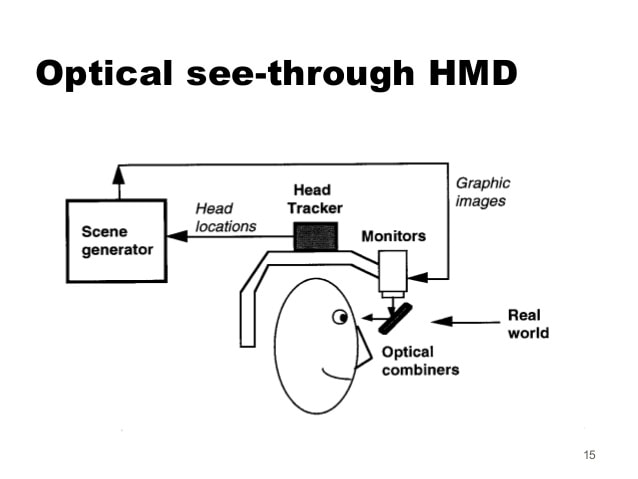
\includegraphics[scale=0.45]{optical-seethrough-screen}
    \caption{Imagen que muestra un esquema de como funcionan las pantallas opticas transparentes.}
    \label{figura-pantalla-optica}
  \end{figure}

  \newpage

  \item \textbf{Pantallas basadas en proyección}: Estas se encargan de proyectar las imágenes virtuales directamente sobre objetos del mundo real, como se puede ver en la Figura \ref{figura-pantalla-proyeccion}, esto combinado con el seguimiento de la posición del usuario y del objeto 3D, permite una aumentación interactiva. Por lo general, estos dispositivos suelen incluir un proyector montado en el techo o paredes.

  \begin{figure}[h]
    \centering
    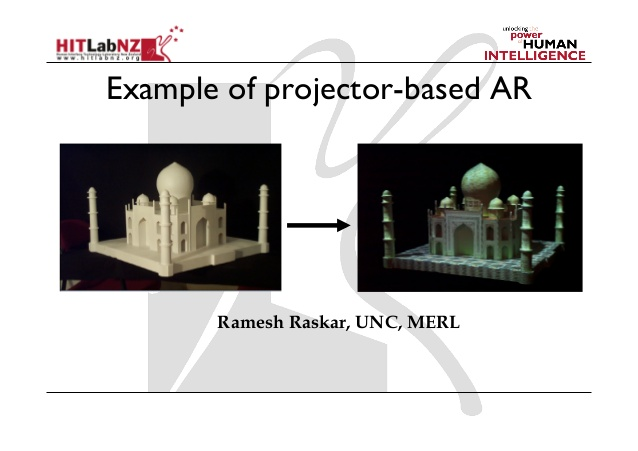
\includegraphics[scale=0.45]{projection-screen}
    \caption{Imagen que muestra como sobre un objeto se proyecta para conseguir una apariencia de objeto real.\protect\footnotemark}
    \label{figura-pantalla-proyeccion}
  \end{figure}

  \footnotetext{{\tt 2013 426 Lecture 2: Augmented Reality Technology. [Diapositivas de Power Point]. Recuperado de }\\
  \url{https://www.slideshare.net/marknb00/2013-426-lecture-2-augmented-reality-technology}. {\tt Billinghurst, M. (23 de julio de 2013).}}

  \item \textbf{Pantallas de ojo multiplexado}: Esta pantalla a diferencia de las anteriores no proporciona el mundo real con las imágenes virtuales ya mezcladas, si no que le proporciona al usuario ambas vistas y es el usuario el encargado de combinarlas mentalmente. Normalmente estas pantallas se suelen situar bastante cerca del ojo del usuario, para facilitar así la integración de los elementos virtuales que la pantalla muestra en el mundo real. Un ejemplo de visión con este tipo de pantallas se puede observar en la Figura \ref{figura-ojo-multiplexado}.

  \begin{figure}[h]
    \centering
    
\includegraphics[scale=0.2]{multiplexed-eye}
    \caption{Imagen que muestra como es llevar las Google Glass puestas.\protect\footnotemark}
    \label{figura-ojo-multiplexado}
  \end{figure}

  \footnotetext{ \url{https://www.youtube.com/watch?v=d-y3bEjEVV8}, Phandroid}

\end{itemize}

\newpage

\begin{flushleft}
Otra forma de categorizar los tipos de pantalla puede ser la siguiente:
\end{flushleft}

\begin{itemize}
  \item \textbf{Head-attached displays}: Son dispositivos que van colocados en al cabeza del usuario, y que pueden ser desde el tamaño de un casco al tamaño de unas gafas.

  \item \textbf{Hand-held display}: Son dispositivos que el usuario puede sujetar con las manos, generalmente serán smartphones y tablets.

  \item \textbf{Spatial displays}: Suelen ser pantallas que están colocadas en un dispositivo o habitación, por lo que no permiten mucha movilidad.

\end{itemize}

\begin{flushleft}
Algunos ejemplos de Head-attached displays:
\end{flushleft}

\begin{itemize}
  \item \textbf{Hololens}: Este dispositivo entraría dentro de las pantallas ópticas transparentes, básicamente tienen unas lentes transparentes que permiten ver el mundo real, pero a la vez en estas se proyectan hologramas que se integran perfectamente con el mundo real gracias a los sensores que las gafas llevan integrados.\cite{hololens}

  \item \textbf{Google glass}: Este dispositivo entraría dentro de las pantallas de ojo multiplexado, son unas gafas que tienen un pequeño espejo semi-reflectivo en el que se muestran las imágenes, que al estar cerca del ojo superpone la información sobre el mundo real. \cite{likamwa}

  \item \textbf{Meta glasses}: Este dispositivo entraría dentro de las pantallas ópticas transparentes, funciona igual que las Hololens, con la diferencia de que necesitan estar conectadas a un ordenador para llevar a cabo el procesamiento gráfico. \cite{meta-vision}

  \item \textbf{Magic Leap}: Este dispositivo entraría dentro de las pantallas ópticas transparentes, el funcionamiento de estas gafas es algo especial, dado que la pantalla es capaz de crear campos de luz como los que percibimos del mundo real, para que la visualización de un objeto 3D sea más natural y no canse la vista. \cite{magic-leap}

  \item \textbf{Mira Headset}: Este dispositivo entraría dentro de las pantallas ópticas transparentes, básicamente dispone de unas gafas con cristal reflectivo y un hueco para colocar un smartphone, por lo que se puede ver a través, pero se ve superpuesta la imagen que muestra el dispositivo móvil gracias a la aplicación de la propia empresa. \cite{mira-ar}

\end{itemize}

\section{Desarrollo de realidad aumentada}

\begin{enumerate}
  \item \textbf{Librerías}
  \begin{itemize}
    \item \textbf{ARKit}: Es la librería creada por Apple para llevar la realidad aumentada a los dispositivos iOS que dispongan de la versión 11 o superior, hace uso de tecnologías similares a ARCore para conocer la posición del dispositivo, detectar superficies horizontales, verticales e irregulares y para conocer las condiciones de luz del entorno. \cite{arkit}

    \item \textbf{Vuforia}: Es un SDK de realidad aumentada muy popular que permite desarrollar aplicaciones tanto para Android como para iOS, su funcionamiento consiste en introducir modelos virtuales en diferentes targets u objetivos, que serán detectados por la camara. Estos objetivos pueden ser imágenes planas como la página de una revista o una fotografía sobre las que se puede colocar un modelo virtual, objetos con diferentes superficies planas, en las que cada superficie plana se considera un objetivo diferente, o modelos que a partir de un modelo 3D permite reconocer uno real a través de la cámara, y utilizarlo como objetivo, por ejemplo coches o juguetes. A diferencia de ARCore y ARKit no conoce la posición del dispositivo con respecto al mundo. \cite{vuforia}

    \item \textbf{EasyAR}: Es un SDK de realidad aumentada que permite desarrollar aplicaciones tanto para Android como para iOS, contiene varias API que permiten programar en c, c++, java en caso de hacer la aplicación para Android y swift en caso de hacer la aplicación para iOS, permite la detección de imágenes planas, es decir, fotos o páginas de revista entre otros sobre las que se puede colocar el modelo virtual, permite la detección de varios objetivos simultáneamente y que el reconocimiento de objetivos se haga en la nube, también permite el seguimiento de objetos 3D. A diferencia de ARCore y ARKit no conoce la posición del dispositivo con respecto al mundo. \cite{easyar}

    \item \textbf{Wikitude}: Es un SDK de realidad aumentada muy reconocida que permite desarrollar aplicaciones tanto para Android, iOS y smartglasses. Incluye en un mismo SDK ARCore y ARKit con su propia plataforma. Permite el reconocimiento de objetos, de imágenes, sobre las que permite colocar un modelo virtual, también permite la geolocalización y el reconocimiento en la nube. A diferencia de ARCore y ARKit no conoce la posición del dispositivo con respecto al mundo. \cite{wikitude}
  \end{itemize}
  \item \textbf{Herramientas de autor}
  \begin{itemize}
    \item \textbf{AR Studio}: Es una herramienta desarrollada por Facebook que te permite crear efectos/elementos que se pueden aplicar al mundo real cuando usas la cámara, es capaz de seguir varios puntos en una cara y de detectar superficies planas, lo que permite aplicar dichos efectos/elementos a esos puntos. La forma de crear estas experiencias de realidad aumentada es mediante un editor gráfico, lo que facilita el proceso. \cite{ar-studio}

    \item  \textbf{Layar}: Es una herramienta desarrollada por la propia empresa Layar, que permite de una forma sencilla crear experiencias de realidad aumentada a partir de una imagen que tu cargas, y la forma de crear esa experiencia es con un editor gráfico. Por ejemplo, puedes poner la imagen de una tarjeta de felicitación y con el editor crear los elementos de realidad aumentada que surgirán a partir de la tarjeta. \cite{layar}
  \end{itemize}

  \item \textbf{ARCore}: Es la librería creada por Google para llevar la realidad aumentada a los dispositivos android que dispongan de la versión 7 o superior, esta librería se basa en el uso de tres tecnologías, motion tracking para que el telefono conozca cuál es su posición relativa al mundo real, environment understanding para que el teléfono detecte la posición y tamaño de superficies horizontales planas y light estimation para que el teléfono pueda conocer las condiciones de luz del entorno.\\

  La tecnología motion tracking que utiliza le permite a través de la camara identificar puntos interesantes del mundo y ver cómo estos puntos se mueven con el tiempo. Y combinando el movimiento de dichos puntos y los sensores del teléfono puede determinar la posición y orientación del teléfono conforme este se mueve por el espacio.\\

  Además de estos puntos de interés, ARCore detecta superficies planas, que junto con la estimación de luz le permiten construir su propia representación del mundo.\\

  Esta representación del mundo permite situar información como objetos, anotaciones, etc. que se integra perfectamente en el mundo real.\cite{arcore}\\

  Elementos destacables de ARCore:

  \begin{itemize}
    \item \textbf{Augmented Images}: Permite a una aplicación que hace uso de la tecnología ARCore, detectar imágenes 2D en el mundo real y sabe las posiciones de estas, es decir, sabe dónde está cada imagen escaneada con respecto al mundo real, por lo que puedes moverte, y la aplicación seguirá teniendo el conocimiento de que está ahí situada esa imagen. Y a una imagen puedes asociar elementos 3D, que se situarán donde el desarrollador indique con respecto a la posición de la imagen a la que están asociados, por lo que, una vez detectada puedes moverte que los elementos 3D mostrados seguirán en esa posición aunque la imagen desaparezca de cámara, ya que, como se ha explicado mantiene la posición de dicha imagen, y por tanto, de sus elementos asociados con respecto al mundo real. Se puede utilizar desarrollando con Android, Android NDK, Unity y Unreal Engine. \cite{arcore-augmented-images}

    \item \textbf{Cloud Anchors}: Permite a una aplicación que hace uso de la tecnología ARCore, compartir Anchors entre distintos dispositivos. Un Anchor describe una ubicación fija y una orientación en el mundo real, por lo que, se puede usar para entonces enlazar objetos a ese anchor, de forma que ese objeto tomará esa posición en el mundo y esa orientación y no se modificará, aportando así una mayor sensación de realismo\cite{arcore-anchors}. Por tanto, al compartir estos anchors, si desde otro dispositivo escaneas la misma escena, va a ser capaz de posicionar dicho anchor en el dispositivo actual, y mostrar los elementos enlazados a dicho anchor en el dispositivo, permitiendo así crear experiencias compartidas. Este componente está disponible tanto para Android como para iOS, de forma que un juego desarrollado para diferentes sistemas operativos pueda compartir esta información, fundamental para las experiencias de realidad aumentada compartidas. Se puede utilizar desarrollando con Android, Android NDK, Unity y Unreal Engine. \cite{arcore-cloud-anchors}

    \item \textbf{Sceneform}: Permite a una aplicación que utiliza ARCore trabajar con dicha tecnología sin necesidad de tener conocimientos acerca de gráficos 3D y OpenGL. Sceneform añade un plugin a Android Studio que permite importar, ver y construir modelos 3D, y también añade una API de alto nivel para los gráficos de escena, todo esto integrable de forma sencilla con ARCore de forma que es sencillo hacer aplicaciones de realidad aumentada. \cite{arcore-sceneform}

  \end{itemize}

  Actualmente ARCore tiene soporte para desarrollo en las siguientes plataformas:

  \begin{itemize}
    \item \textbf{Android}: Se utilizará el framework “Android Studio”, y el lenguaje Java.

    \item \textbf{Android NDK (Kit de desarrollo nativo)}: Se utilizará el framework “Android Studio”, y el lenguaje C o C++. Android NDK consiste en un conjunto de herramientas que te permiten utilizar código C o C++ en aplicaciones Android, de forma que, por ejemplo, puedes utilizar bibliotecas que ya tenias, mejorar el rendimiento de la aplicación o conectar una aplicación entre plataformas. \cite{ndk}

    \item \textbf{iOS}: ARCore permite que mientras se desarrolla utilizando ARKit, mediante la SDK que proporcionan puedas utilizar anchors que otro dispositivo ha creado, usando la característica “Cloud Anchor”, o crear esos anchors y compartirlos.

    \item \textbf{Unity}: Permite el desarrollo de videojuegos con Unity utilizando el SDK de ARCore para esta plataforma, la programación de los scripts característicos de Unity se llevará a cabo utilizando el lenguaje C# o UnityScript, lenguaje que fue creado con JavaScript como base. \cite{unity-scripting}

    \item \textbf{Unreal Engine}: Permite el desarrollo de videojuegos con Unreal Engine utilizando el SDK de ARCore para esta plataforma, la programación en Unreal se lleva a cabo utilizando el lenguaje C++. \cite{unreal}

    \item \textbf{Web}: Permite el desarrollo web utilizando Realidad Aumentada, de forma que usando la librería javascript “three.ar.js”, y un navegador especial para realidad aumentada que ellos proporcionan, se puede utilizar la realidad aumentada en tecnologías web. \cite{arcore-web}
  \end{itemize}

\end{enumerate}

\section{Interfaces tangibles}
Las interfaces tangibles son interfaces de usuario mediante las cuales el usuario interactúa con la información digital a través del entorno físico. \cite{ullmer}\\

El mayor ejemplo de interfaz tangible es el ratón, en el caso de la realidad aumentada la interfaz tangible consiste en un elemento, que al entrar dentro del rango de la cámara se convierte en un elemento que puede modificar la información virtual que se está mostrando en la pantalla.\\

Como ejemplo de interfaces tangibles en realidad mixta tenemos los “Motion controllers” del kit “Microsoft Mixed Reality”, son dos mandos que al ser reconocidos por los sensores del casco permiten modificar elementos virtuales. \cite{windows-mixed-reality}\\

Como ejemplo de interfaces tangibles en realidad aumentada tenemos ARtalet, es un proyecto que permite reconocer la posición de un ratón puntero por unas pegatinas en la punta de éste, y recibe señales de los botones del ratón, y con este puntero que reconoce la camara son capaces de manipular otros elementos virtuales que se habían situado en el entorno real que la cámara percibe. \cite{ha}\\

\chapter{Metodologías utiliazdas para el desarrollo}
\label{ch:metodologia}

\chapter{Proceso de desarrollo}
\label{ch:desarrollo}

\chapter{Resultados y Conclusiones}
\label{ch:conclusiones}

\chapter{Anexos}
\label{ch:anexos}


% Glosario de términos
\backmatter
\begingroup
	\setlength\parindent{0pt}
	\chapter{Glosario de términos}

\begin{description}
  
\end{description}

\endgroup

% Bibliografía
\newpage
\begin{thebibliography}{99}
	\addcontentsline{toc}{chapter}{Bibliografía}

\subsection*{Páginas web consultadas durante la realización del proyecto}

\bibitem{globalizacion} {\tt Globalización - Wikipedia}\\
\url{https://es.wikipedia.org/wiki/Globalizaci%C3%B3n}

\bibitem{globalreport} {\tt Globalization Report 2016 - Who benefits most from globalization?}\\
\url{https://www.bertelsmann-stiftung.de/fileadmin/files/BSt/Publikationen/GrauePublikationen/NW_Globalization_Report_2016.pdf}

\bibitem{internetusage} {\tt Wikipedia - Global Internet usage stats from the International Telecommunications Union}\\
\url{https://en.wikipedia.org/wiki/Global_Internet_usage#Internet_users}

\bibitem{ugremprende} {\tt UGR Emprendedora - Página principal}\\
\url{https://ugremprendedora.ugr.es/}

\bibitem{h2020} {\tt Horizon 2020 - Página principal}\\
\url{https://ec.europa.eu/programmes/horizon2020/}

\bibitem{agilereport} {\tt Top 10 Insights from the 11th Annual State of Agile Report}\\
\url{https://explore.versionone.com/state-of-agile/top-10-insights-from-the-11th-annual-state-of-agile-report-2}

\bibitem{health1} {\tt PubMed Central - Multidisciplinary in-hospital teams improve patient outcomes: A review}\\
\url{https://www.ncbi.nlm.nih.gov/pmc/articles/PMC4173201/}

\bibitem{health2} {\tt PubMed Central - Benefits of multidisciplinary teamwork in the management of breast cancer}\\
\url{https://www.ncbi.nlm.nih.gov/pmc/articles/PMC3929250/}

\bibitem{neuroped} {\tt Imagen original de NeuroPed - Enlace}\\
\url{http://www.neuroped.es/equipo-multidisciplinar/}

\bibitem{medialabugr} {\tt Medialab UGR - Página principal}\\
\url{http://medialab.ugr.es/}

\bibitem{linkuma} {\tt Link by UMA-ATech (Universidad de Málaga) - Página principal}\\
\url{http://www.link.uma.es/}

\bibitem{linkimage} {\tt Fotografía original de Geek and Tech Girls}\\
\url{https://geekandtechgirls.github.io/We-Create-Technology/}

\bibitem{linkedin} {\tt LinkedIn - Página principal}\\
\url{https://es.linkedin.com/}

\bibitem{kickstarter} {\tt Kickstarter - Página principal}\\
\url{https://www.kickstarter.com/}

\bibitem{responsivelink} {\tt Página de inicio de \textit{Responsive Web Design}}\\
\url{https://responsivedesign.is/}

\bibitem{contentwater} {\tt Imagen original de Wikimedia - Enlace}\\
\url{https://commons.wikimedia.org/wiki/File:Content_is_like_water.png}

\bibitem{framework} {\tt Framework - Wikipedia}\\
\url{https://es.wikipedia.org/wiki/Framework}

\bibitem{startup} {\tt Startup - Wikipedia}\\
\url{https://es.wikipedia.org/wiki/Empresa_emergente}

\bibitem{designthinkinglink} {\tt Design Thinking en Español - Página oficial}\\
\url{http://designthinking.es/inicio/index.php}

\subsection*{Libros consultados}

\bibitem{gangoffour}
Gamma, E., Helm, R., Johnson, R. and Vlissides, J. 1994. {\em Design Patterns. Elements of Reusable Object-Oriented Software}. Addison Wesley.

\bibitem{brandon}
M. Brandon, D. 2008. {\em Software Engineering for Modern Web Applications: Methodologies and Technologies}. Information Science Reference.

\bibitem{pressman}
Pressman, R. 1982. {\em Software Engineering - A Practitioner's Approach}. McGraw-Hill Higher Education.

\bibitem{pressmanweb}
Pressman, R. and Lowe, D. 2009. {\em Web Engineering - A Practitioner's Approach}. McGraw-Hill Higher Education.

\bibitem{headfirstpatterns}
Sierra, K., Freeman, E., Robson, E. and Bates, B. 2004. {\em Head First Dessign Patterns. A Brain-Friendly Guide}. O'Reilly.

\subsection*{Páginas de principales productos y programas usados}

\bibitem{bootstrap} {\tt Bootstrap Framework - Página principal}\\
\url{https://getbootstrap.com/}

\bibitem{laravel} {\tt Laravel - Página principal}\\
\url{https://laravel.com}

\bibitem{xampp} {\tt XAMPP - Página oficial}\\
\url{https://www.apachefriends.org/es/index.html}

\bibitem{slack} {\tt Slack - Página oficial}\\
\url{https://slack.com/}

\bibitem{googlecalendar} {\tt Google Calendar - Página oficial}\\
\url{https://www.google.com/calendar}

\bibitem{googledrive} {\tt Google Drive - Página oficial}\\
\url{https://www.google.com/drive}

\bibitem{whatsapp} {\tt WhatsApp - Página oficial}\\
\url{https://www.whatsapp.com/}

\subsection*{Otros recursos utilizados}

\bibitem{laraveldocs} {\tt Documentación oficial de Laravel 5.5}\\
\url{https://laravel.com/docs/5.5/}

\bibitem{bootstrapdocs} {\tt Documentación oficial de Bootstrap 3.3}\\
\url{https://getbootstrap.com/docs/3.3/}\\

Apuntes de asignaturas del \textbf{Grado en Ingeniería Informática}, tales como:
\begin{itemize}
    \item Desarrollo de Aplicaciones para Internet
    \item Sistemas de Información Basados en Web
    \item Desarrollo de Software
    \item Fundamentos de Ingeniería del Software
    \item Dirección y Gestión de proyectos
    \item Metodologías de Desarrollo Ágil
    \item Diseño y Desarrollo de Sistemas de Información
\end{itemize}

\end{thebibliography}

\chapter*{}
\thispagestyle{empty}

\end{document}
